% !TEX encoding = UTF-8 Unicode
%\documentclass[12pt,reqno]{amsart}
\documentclass{article}
%\usepackage{tocloft}

%\cftsetindents{section}{0.5in}{0.5in}
%\cftsetindents{subsection}{0.5in}{0.5in}
\usepackage[utf8]{inputenc}
%\usepackage[dvips]{graphicx,graphics}
\usepackage{enumitem}
\usepackage{listings}
\usepackage{xcolor}
\definecolor{dkgreen}{rgb}{0,0.6,0}
\definecolor{gray}{rgb}{0.4,0.4,0.4}
\usepackage{graphicx}
\usepackage{euscript}
\usepackage{graphics}
%\usepackage{russcorr}
\usepackage[active]{srcltx} % SRC Specials: DVI [Inverse] Search
\usepackage{amssymb,amsmath,amsthm,amsfonts}
\usepackage{amsopn}

\usepackage{verbatim}
\usepackage{hyperref}
\hypersetup{
    colorlinks,
    citecolor=black,
    filecolor=black,
    linkcolor=blue,
    urlcolor=blue
}
\usepackage{titlesec}
\titleformat{\section}[block]{\color{blue}\Large\bfseries\filcenter}{\thesection.}{1em}{}
\titleformat{\subsection}[hang]{\color{blue}\large\filcenter}{\thesubsection.}{1em}{}

\setlist[itemize,1]{leftmargin=\dimexpr 26pt+.3in}
\usepackage{a4wide}
\lstset{language=C++,
                basicstyle=\ttfamily,
		frame=tb,
		  aboveskip=3mm,
		  belowskip=3mm,
		  numberstyle=\tiny\color{gray},
		  keywordstyle=\color{blue},
		  commentstyle=\color{dkgreen},
		  stringstyle=\color{mauve},
		  breaklines=true,
		  breakatwhitespace=true,
		  tabsize=3,
                morecomment=[l][\color{magenta}]{\#}
}
\begin{document}

\begin{center} \hyperref[debug]{\Huge{debug}}\end{center}
\begin{center}
 \Large{\bf RAST: highly distributed DB project.}

{\large {\bf Produced by NOA team}}
\end{center}

\tableofcontents

\newpage
\section{Algorithmic basis}

\subsection{Free-list multi-level allocator}
\label{free_list_algo}

On of the most important steps in order to make a low-latency system is to consider the allocation problem. The problem is that sometimes different components of the program require very small parts of memory to be allocated. Asking the system to allocate memory directly would result in slower performance. That's why it is better to allocate large memory segment and distribute its parts among several consumers.

But here we face another difficulty, so called fragmentation problem. Imagine that an allocated segment is separated into several parts owned by consumers. Some time after, some of the consumers returned their own parts to allocator (calling deallocate method). Afterwards it appears that the returned memory in control of allocator is represented as distinct small fragments. Those fragments cannot be given to a consumer, who asks for a larger memory segment, than the size of the separate fragment. If there is a lot of such unusable fragments, we would have a lot of memory allocated, which will never be used. In order to avoid this problem, we have to force each small fragment to be used by a consumer who asks for a small amount of memory.

The main idea is to use a memory levels.

\begin{center}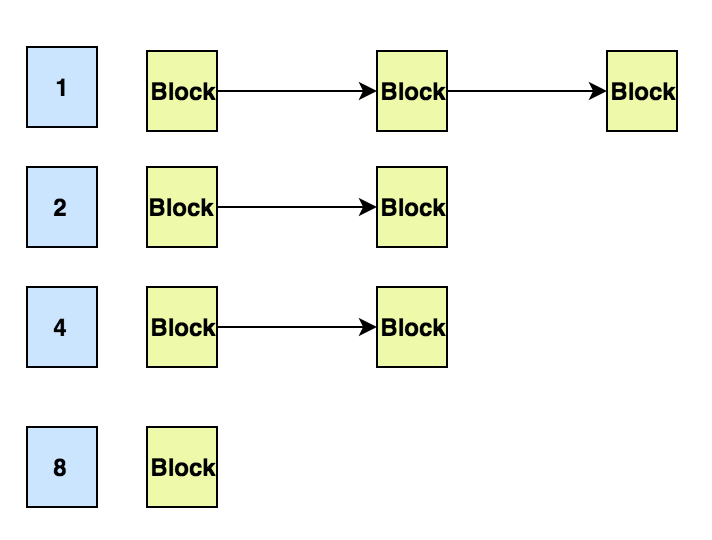
\includegraphics[width=0.5 \textwidth]{image1.png}\end{center}

For each block size we calculate an integer part of $log(size)$ and put all blocks of memory in the corresponding list.

By means of the list, we can easily find the block of needed size and remove (detach) it from the list, giving ownership to the consumer, who asked to allocate memory. Likewise, when a consumer asks to deallocate the block, we may put (attach) it again in the list.

Also we want to join small segments of memory returned by consumers to one large segment in case if they go one after another in the global memory space. In order to do this, let us have the following structure of the memory block:

\begin{center}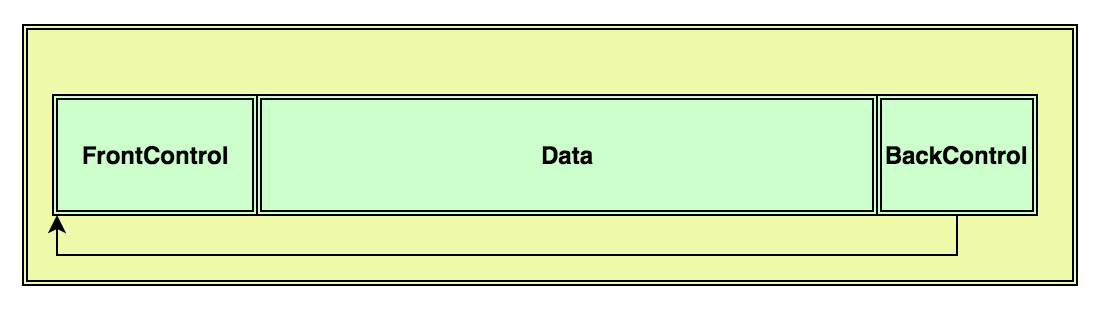
\includegraphics[width=0.5 \textwidth]{image2.png}\end{center}

The block will consist of three logical parts:
\begin{itemize}
\item FrontControl, which stores the $data\_size$ which is size of the block, $localnext$ and $localprev$ pointers, $offset$ in external allocated segment, and $total\_size$ of external segment, and $is\_owned$ -- whether the block is owned by the allocator itself or was it given away to the consumer.
\item Data -- raw byte space, which would be given an external consumer to control
\item BackControl, which stores pointer to the FrontControl (pointer to the beginning of the entire block)
\end{itemize}

$localprev$ and $localnext$ pointers will help us to build freelists, which were described above. BackControl block will help us to find the block, previous to some specific Block, so that we could join two blocks together in case they both have been returned to the allocator. Here is how joining procedure works:

\begin{center}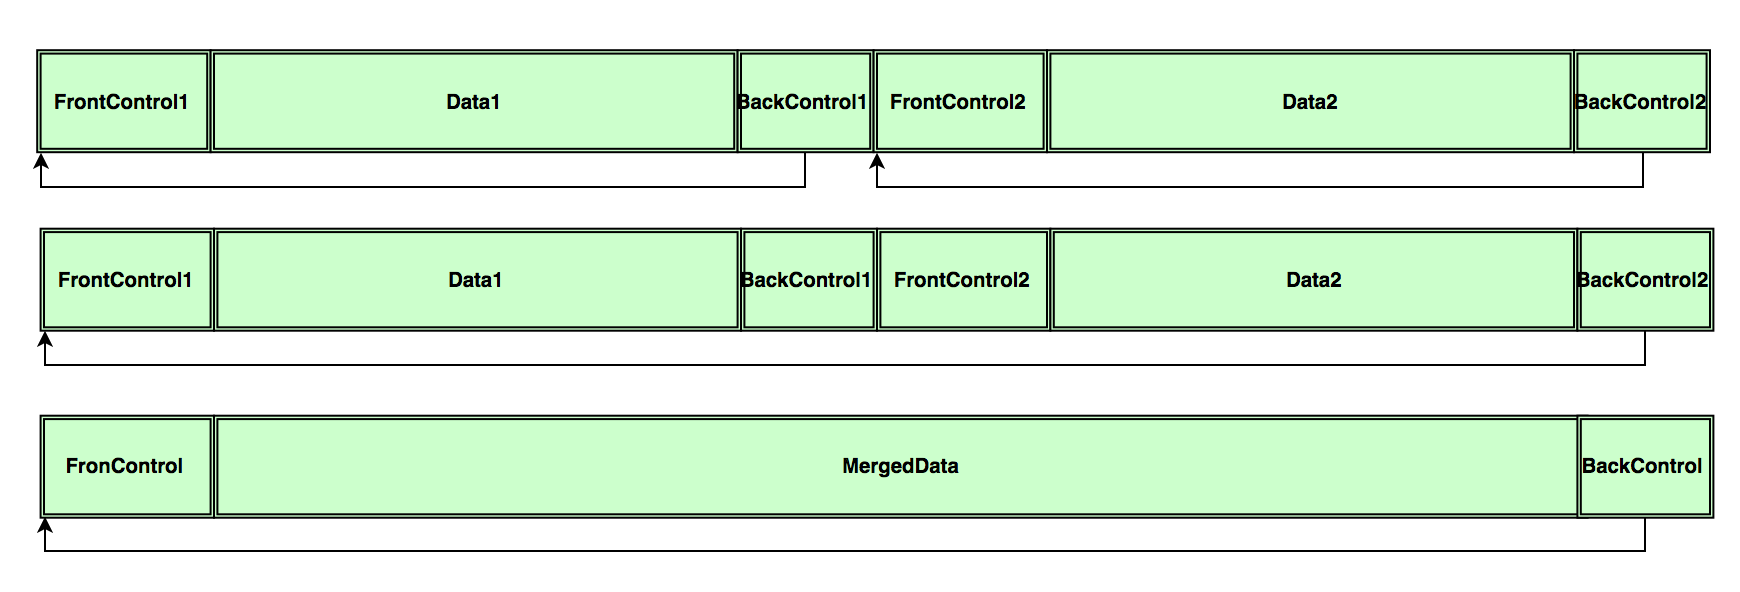
\includegraphics[width=1 \textwidth]{image3.png}\end{center}

The steps are very simple:

\begin{itemize}
\item detach first block from its list
\item detach second block from its list
\item point BackControl2 to FrontControl1
\item change FrontControl1 information about block size
\item do nothing about BackControl1 and FrontControl2, because now we threat them as a garbage part of MergedData, and we do not have to care about their contents so far
\item attach new merged block to its new list (based on $log(size)$ where $size$ is a sum of sizes of these two blocks) by changing $localprev$ and $localnext$ pointers of FrontControl.
\end{itemize}

Also, one can easily imagine how to split one large block into two smaller.

Blocks contained in the same external memory segment (which allocator asked from the system) may be joined and split so that we know exactly how many consequent free to use bytespace fragments do we have.

Finally, the allocation procedure is the following:

\begin{itemize}
\item calculate integral part $N = int(log(size))$ of the size of the memory consumer asks to allocate
\item if the corresponding $N$-th list of blocks is empty, we allocate several external blocks of the sizes $2^{N}$ and build Block structure upon each of them, putting blocks to the $N$-th list
\item detach first block from the list
\item split the block into two blocks: first block has exactly needed size, second block consists of what is remained
\item attach second block to its corresponding list
\item mark the first block as not owned by allocator
\item return a pointer to the Data section of the first block to a consumer
\end{itemize}

The deallocation procedure:
\begin{itemize}
\item receive from a consumer a pointer to deallocate data
\item calculate the pointer to FrontControl (by subtracting $sizeof(FrontControl)$ from Data pointer)
\item mark block as owned by the allocator
\item read $offset$ from FrontControl, if $offset > 0$, than there is some previous block in the external memory segment.
\item calculate the pointer to BackControl of the previous block (by subtracting $sizeof(BackControl)$ from the pointer to the current block)
\item get the pointer to the FrontControl of the previous block via BackControl
\item check whether the previous block is owned by the allocator and if it is, merge it with the current block
\item if $offset < total\_size$ where $total\_size$ is the size of external allocated memory segment, we may want to check whether we can merge with the forthcoming block
\item calculate the pointer to the FrontControl of the forthcoming block (by adding $data\_size + sizeof(FrontControl) + sizeof(BackControl)$ to the pointer to the current block)
\item check if the forthcoming block is owned by allocator using its FrontControl and if it is, merge it with the current block.
\end{itemize}
\newpage

\subsection{Multi-reference counting lock-free queue}
\label{lock_free_queue}

Queue is a basic container, which is often desired to be used in more or less complicated systems. Although queue implementation is very simple, it is not thread-safe. In order to make it thread-safe, one may decide to use mutexes in Pop and Push operations. The idea is not good enough for several reasons:
\begin{itemize}
	\item all threads would compete against each other for gaining control over mutex,
	\item all kernels would have to sync the mutex state via cache ping-pong, which would lead to plenty of time waisted on system calls,
	\item jobs of threads would be serialized, that is, the queue is 100\% not scalable.
\end{itemize}

The main idea is that if we get down to the details of queue implementation, we may reorganize it in such a way, that we would not need to have mutual exclusive access to guarantee that each operation works fine. That is, we may obtain a lock-free algorithm on the queue.

In order to do that, let us represent queue as a linked list, each node of each except for the last one, contains data elements. The last node, which is the tail of the queue would not contain any data at all. Let us call it a dumb node:

\begin{center}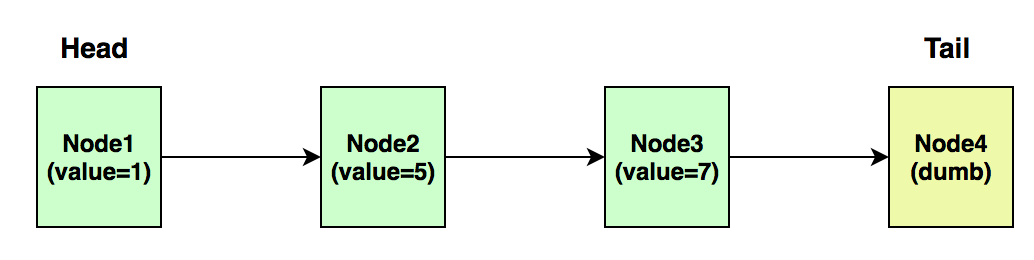
\includegraphics[width=0.5 \textwidth]{image4.png}\end{center}

Head, Tail and Next pointers inside data structure would be atomic pointers, which would be changed using CAS operations. The main idea of Push is:
\begin{itemize}
	\item put new data to the dumb node
	\item create another dumb node and mark it as a tail
\end{itemize}

But these are two distinct actions, which are not guarded by mutual exclusion and thus are not atomic. So, by choosing this strategy we should agree that it is OK for the queue to be one of the following two:

\begin{center}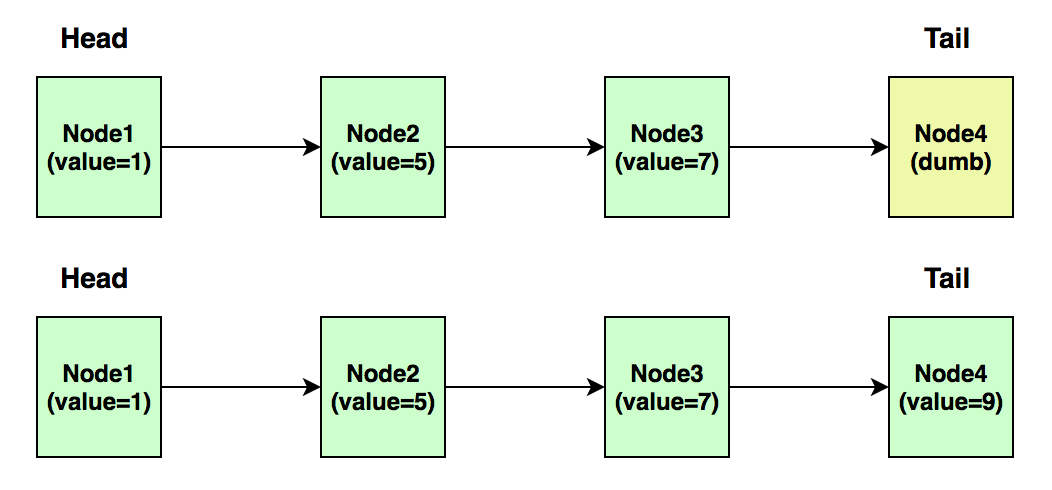
\includegraphics[width=0.5 \textwidth]{image5.png}\end{center}

That is, we agree on purpose that queue may either have dumb element or not have dumb element. But if it is like that, we have to redesign Push:
\label{debug}
\begin{itemize}
	\item try CAS data on the tail (nullptr $\rightarrow$ our new data)
	\item if CAS succeeded, the queue actually had a dumb node and now we may proceed to adding a new dumb node
	\item if CAS failed, the queue does not have a dumb element, so we firstly create a dumb node as a tail, and retry the algorithm from the start
\end{itemize}

Changing tail pointer is also a CAS operation, but in case if it fails, we realize that another thread have already moved tail forward and thus we do not have to do anything, so we will not process tail CAS operation failure on purpose without harming algorithm invariants at all.

The detailed version of Push consists of the following steps:
\begin{itemize}
	\item allocate new data
	\item allocate new dumb node
	\item L1: load tail
	\item L2: try CAS tail.data (nullptr $\rightarrow$ allocated new data)
	\item L3: if L2 succeeded, try CAS tail.next (nullptr $\rightarrow$ new dumb node)
	\item if L3 failed, somebody already moved tail to new node, so deallocate new dumb node and finish
	\item if L3 succeeded, try CAS tail old\_tail $\rightarrow$ new dumb node, do not care about results
	\item L4: if L2 failed, we do not have dumb node in the end of the queue, try CAS tail$\rightarrow$next (nullptr $\rightarrow$ new dumb node)
	\item if L4 succeeded, we shall allocate new dumb node and repeat algorithm from L1 point
	\item if L4 failed, we repeat algorithm from L1 point using the same already-allocated new dumb node
\end{itemize}

Note that the only action among these which may throw is an allocation, but all allocations happen-before successful L2 step. That is, in case if L2 succeeded, the rest of the code in Push in exception-free. Success of L2 operation means that new data is put to the queue, failure means that the data was not put to the queue yet. This implies we are having strong exception safety on Push operation: if it throws, it would surely mean that data was not put to the queue. This is the best available exception guarantee (after "noexcept") for a queue user. Of course, guaranteeing noexcept is impossible, because no one can imagine Push operation without memory allocations, which always may throw.

Now let us consider Pop operation. It would check if head is equal to tail. If it is, the queue consists of dumb node only, thus there is no data. In this cast Pop would return empty unique\_ptr. In the other case, we will switch the head to the next element, giving away first node data.

The detailed version of Pop consists of the following steps:
\begin{itemize}
	\item read head, tail
	\item L1: check head == tail
	\item if L1 is true, return empty unique\_ptr
	\item L2: if L1 is false, do CAS head (current, next)
	\item if L2 failed, retry from the start
	\item if L2 succeeded, store and exchange data from old head, return it to the caller
\end{itemize}

\section{Detailed Code Architecture (classes and methods)}

\subsection{TLS free-list multi-level allocator}

The class implements the allocation logic described \hyperref[free_list_algo]{here}.

\begin{lstlisting}
class FreeListMultiLevelAllocator {
	FreeListMultiLevelAllocator()
	// Exceptions:
	// 	may throw, strong exception safety

	FreeListMultiLevelAllocator(
		const FreeListMultiLevelAllocator&) = delete;

	FreeListMultiLevelAllocator(
		FreeListMultiLevelAllocator&&) = delete;

	FreeListMultiLevelAllocator& operator=(
		const FreeListMultiLevelAllocator&) = delete;
	// We will use object as s singleton, no copying and assigning

	template <typename T>
	T* Allocate(const size_t size);
	// Return value:
	// 	a pointer to allocated block
	// Exceptions:
	// 	may throw std::bad_alloc
	// 	strong exception safety: no side effects in exception case

	template <typename T>
	void Deallocate(T* pointer, const size_t size) noexcept;
};

thread_local FreeListMultiLevelAllocator global_allocator;
// Memory allocations would be controlled by this TLS singleton

template <typename T>
class FixedFreeListMultiLevelAllocator<T> {
	FixedFreeListMultiLevelAllocator() noexcept;

	FixedFreeListMultiLevelAllocator(
		const FixedFreeListMultiLevelAllocator&) noexcept;

	template <class U>
	FixedFreeListMultiLevelAllocator(
		const FixedFreeListMultiLevelAllocator<U>&) noexcept;
	// These three methods are empty,
	// 	they are needed for compatibility with std::allocator

	T* allocate(const size_t n);
	// Calls global_allocator.Allocate<T>(n)
	// Return value:
	// 	a pointer to allocated block
	// Exceptions:
	// 	may throw std::bad_alloc
	// 	strong exception safety: no side effects in exception case

	void deallocate(T* p, const size_t n) noexcept;
	// Calls global_allocator.Deallocate<T>(p, n)
};
\end{lstlisting}

\subsection{Lock-free queue}

$LockFreeQueue<TElement>$ is an implementation of lock-free queue described \hyperref[lock_free_queue]{here}. It contains the following functions:

\begin{lstlisting}
class LockFreeQueue<TElement> {
	void Push(TElement new_element);
	// Exceptions:
	// 	Strong exception safety: in case of failure
	// 	the element is not pushed to the queue,
	// 	there are no visible side effects

	std::unqiue_ptr<TElement> Pop() noexcept;
	// Return value:
	// 	nullptr unique_ptr if the queue was empty,
	// 	unique_ptr pointing on TElement in case of successful pop
};
\end{lstlisting}

\end{document}

